% =====================================================================
%  The D'Agnese Chart Operator
%  A certified, adaptive chart for neural operators on deformed meshes
%
%  Build:  pdflatex dagnese-chart-operator && bibtex dagnese-chart-operator
%          && pdflatex ... (twice)
%  or:     latexmk -pdf dagnese-chart-operator.tex
% =====================================================================
\documentclass[11pt,a4paper]{article}

\usepackage[T1]{fontenc}
\usepackage[utf8]{inputenc}
\usepackage{lmodern}
\usepackage[margin=2.4cm]{geometry}
\usepackage{amsmath,amssymb,amsthm,mathtools}
\usepackage{booktabs,multirow,array}
\usepackage{graphicx}
\usepackage{xcolor}
\usepackage{algorithm}
\usepackage{algpseudocode}
\usepackage[colorlinks=true,linkcolor=blue!50!black,citecolor=blue!50!black,
            urlcolor=blue!50!black]{hyperref}
\usepackage{cleveref}

\theoremstyle{plain}
\newtheorem{theorem}{Theorem}
\newtheorem{proposition}[theorem]{Proposition}
\newtheorem{lemma}[theorem]{Lemma}
\newtheorem{corollary}[theorem]{Corollary}
\theoremstyle{definition}
\newtheorem{definition}[theorem]{Definition}
\newtheorem{remark}[theorem]{Remark}

\newcommand{\R}{\mathbb{R}}
\newcommand{\Id}{\mathrm{Id}}
\newcommand{\dd}{\,\mathrm{d}}
\newcommand{\transp}{\mathsf{T}}
\newcommand{\detJ}{\det J_\Phi}
\newcommand{\Leq}{\mathcal{L}_{\mathrm{eq}}}
\newcommand{\Om}{\Omega_{\mathrm{ref}}}
\newcommand{\Pa}{P_{\Phi}}
\newcommand{\DAO}{\textsc{D'Agnese Chart Operator}}
\newcommand{\code}[1]{\texttt{#1}}

\title{\bfseries The D'Agnese Chart Operator:\\[2pt]
Certified, Exactly Invertible, Adaptively Learned Charts\\[2pt]
for Neural Operators on Deformed Meshes}

\author{Giovanni D'Agnese\thanks{Code: \url{https://github.com/GiovanniDAgnese-paper/DIF-FNO}.}}

\date{Preprint. \today}

\begin{document}
\maketitle

\begin{abstract}
Neural operators such as the Fourier Neural Operator (FNO) learn maps between
function spaces on a \emph{fixed} grid.  Deforming that grid — evaluating the
operator on a learned chart — is an old idea with a fatal defect: a neural
network that produces the deformation has no guarantee of producing a
\emph{diffeomorphism}, and a folded chart silently destroys the representation
(negative or vanishing Jacobian determinant), usually without any symptom in the
training loss.  Existing remedies penalise folding; none removes it.

We introduce the \emph{D'Agnese chart}, a constructive class of maps
$\Phi(\xi_1,\xi_2)=(g(\xi_1),h(\xi_1,\xi_2))$ generated by strictly positive
increments, for which global injectivity, orientation ($\detJ>0$ everywhere) and
a \emph{closed-form} inverse hold by construction, for every parameter value,
with an explicit parameter-free lower bound $\detJ\ge\varepsilon^2$ that does not
degrade as the deformation grows.  We embed it in the \emph{\DAO{} (DAO)}, which
is \emph{exactly} the FNO baseline at initialisation and therefore a strict
super-set of it; and we introduce the \emph{D'Agnese Equidistribution Loss}, the
normalised variance of the monitor mass per cell, which vanishes exactly on
equidistributing meshes, is scale free, controls the worst cell through
$\max_C M_C/\bar M\le 1+\sqrt{N_c\Leq}$, and minimises a certified upper bound on
the representation error at fixed resolution.

We verify the propositions deterministically, not statistically: zero folded
cells across a sweep of chart-parameter scales from the identity to $10^{3}\times$
the initialisation scale; a pullback/pushforward round trip of observed order
$1.97$; a chart learned by gradient descent on the
equidistribution loss alone that compresses a boundary layer into $1.30$ mass
ratio and reduces the representation error by $4.1\times$.  We also report a
negative result — on a field whose monitor is already uniform, equidistribution
\emph{hurts} ($0.54\times$) — and we explain why that is the expected behaviour
of the objective rather than a defect of the method.  A paired-seed benchmark across six geometries and three seeds closes the gap
between the guarantees and the PDE error: the operator improves the relative
$L^2$ error by $9.3\%$ and the $H^1$ error by $10.2\%$ (pooled paired
differences, $p<10^{-3}$ for both, sixteen of eighteen runs improved, six of six
geometries), with zero folded cells and a positive certificate on every run.
An ablation with the same chart, the same parameters and the same budget
isolates the mechanism: adding the equidistribution loss to the chart improves
seventeen of eighteen runs ($p=4\cdot10^{-4}$).  The effect is real, but modest,
protocol specific, and not implied by the theory; we say so.
\end{abstract}

\tableofcontents

% =====================================================================
\section{Introduction}
% =====================================================================

Learning solution operators of parametric partial differential equations
(PDEs) has become a discipline of its own: DeepONet
\cite{lu2021deeponet,lu2022fair}, the Fourier Neural Operator
(FNO) \cite{li2021fno,kovachki2023neuraloperator}, and physics-informed
variants \cite{raissi2019pinn,sirignano2018dgm,weinan2018deepritz} all replace
the classical solver by an amortised map between function spaces.  Their common
structural assumption is a \emph{fixed} discretisation: the same grid at
training and test time, the same grid for every sample.  That is at once their
strength (resolution transfer comes for free) and their weakness (the grid knows
nothing about the solution).

The classical remedy is an \emph{adaptive mesh}.  The $r$-adaptive (moving mesh)
literature \cite{huang2011moving,budd2009adaptivity,deboor1973good} has known for
fifty years that a mesh which equidistributes a monitor function minimises the
worst cell mass and, under smoothness, a certified upper bound on the
interpolation error \cite{babuska1978error}.  The obvious question — can a neural
operator \emph{learn} such a mesh end to end? — runs immediately into a
geometric obstruction: the mesh must be the image of the reference grid under a
diffeomorphism, and a neural network parametrising that diffeomorphism has no
reason to produce one.

Two lines of work have approached the obstruction.  Deformation-based neural
operators \cite{li2022geofno} learn a single deformation that maps an irregular
physical geometry onto a regular computational one; the deformation is trained
unsupervised so that the boundary is mapped to the box, and it is not certified.
Diffeomorphism penalties (our own earlier DIF-FNO line, and the general
philosophy of \cite{behrmann2019invertible}) add a term that becomes large when
$\detJ\le 0$.  A penalty makes folding \emph{expensive}; it never makes it
\emph{impossible}, and the failure mode is quiet: in our own v1 measurements a
barrier-regularised model folded $21.7\%$ of the cells on the star geometry at a
large deformation scale, while reporting a healthy validation loss.

\paragraph{This paper.}  We replace the penalty by a \emph{class}.  Our
contributions are:

\begin{enumerate}
\item \textbf{The D'Agnese chart} (\Cref{sec:chart}): a constructive family of
  diffeomorphisms of the reference square with global injectivity, $\detJ>0$ as
  a product of positive factors (no cancellation), a closed-form inverse at
  \emph{arbitrary} points, a parameter-free lower bound $\detJ\ge\varepsilon^2$,
  exact identity at initialisation, and closure under composition.  The
  guarantee is structural, not statistical, and holds for every parameter value,
  including the ones an adversarial optimiser would find.
\item \textbf{The \DAO} (\Cref{sec:operator}): an FNO evaluated on the chart.
  At initialisation it reproduces the FNO bit-for-bit ($3\cdot10^{-8}$ measured),
  so it is a strict super-set of the baseline, and it can be conditioned on the
  input field so that the chart is a \emph{mesh model} rather than a single
  mesh.
\item \textbf{The D'Agnese Equidistribution Loss} (\Cref{sec:loss}): the
  normalised variance of the monitor mass per cell.  We prove that it vanishes
  exactly on equidistributing meshes, is scale free, controls the worst cell by
  $\sqrt{N_c\Leq}$, and, through the de Boor–Babuška–Rheinboldt argument,
  minimises a certified upper bound on the representation error.  Gradient
  descent on this loss \emph{alone} learns a classical equidistributing mesh
  without ever seeing a solution.
\item \textbf{A verification protocol} (\Cref{sec:experiments}) that separates
  what is proved from what is measured: deterministic sweeps for the
  certificate and the transport, a learned-mesh experiment with an honest
  negative result, and a paired-seed PDE benchmark whose conclusion is stated
  with its noise.
\end{enumerate}

We are deliberately conservative about the last item.  The guarantee is
topological, not variational: nothing in \Cref{sec:chart,sec:loss} bounds the
PDE error, and the accuracy we measure is a measurement.  What makes it
informative is the ablation --- the same chart, with and without the
equidistribution objective, at the same budget --- which separates ``a learned
deformation'' (the chart alone) from ``an equidistributing one'' (the chart plus
the loss).  \Cref{sec:discussion} says exactly which claims the measurements
support and which they do not.

% =====================================================================
\section{Setting and related work}
\label{sec:related}
% =====================================================================

\paragraph{Neural operators.}  An operator $\mathcal{G}:\mathcal{A}\to\mathcal{U}$
between Banach spaces is approximated by $\mathcal{G}_\theta$ acting on
discretised inputs.  FNO \cite{li2021fno} composes spectral convolutions on the
lowest Fourier modes with pointwise mixing, and is discretisation invariant in
the sense that the same weights act at any resolution.  We take the FNO as the
backbone for concreteness; nothing in \Cref{sec:chart,sec:loss} depends on that
choice.

\paragraph{Deformed meshes.}  Geometry-adaptive convolutional networks
\cite{gao2021phygeonet} and Geo-FNO \cite{li2022geofno} learn a deformation
$\phi$ from the physical geometry to a regular domain and applies the FNO in
computational space, with $\phi$ trained unsupervised to align the boundary.
The transport is the same pullback/pushforward we use; the differences are
(i) our chart maps the \emph{reference square} to itself, so the operator's
domain is unchanged and the identity is in the class, (ii) injectivity is
certified rather than encouraged, and (iii) the chart can be equidistributing,
which is a criterion, not a heuristic.  Our \code{chart-only} variant is the
empirical control for this comparison: a learned deformation, optimised only by
the PDE loss, with no equidistribution prior — a Geo-FNO-like deformation inside
our certified class.  It improves $H^1$ but not $L^2$ significantly
(\Cref{sec:experiments}), so the gain we report is not the gain of ``learning a
deformation'' in general; it is the gain of learning an \emph{equidistributing}
one.

\paragraph{Invertible networks.}  Normalising flows \cite{rezende2015variational,
dinh2017density}, continuous-time flows \cite{chen2018neuralode} and invertible
residual networks \cite{behrmann2019invertible}
establish invertibility by construction, either through triangular/coupling
structure or through a Lipschitz constraint.  Our chart is a triangular
construction in the same spirit — a coupling architecture whose two coordinate
maps are monotone — transferred from density estimation to \emph{mesh geometry}.
Two differences matter: the Lipschitz route requires $\kappa L<1$, i.e. a
neighbourhood of the identity, and a neighbourhood cannot represent a strong
mesh deformation; and we need $\detJ$ \emph{positivity} together with an
explicit bound, which we obtain from the increment representation.

\paragraph{Adaptive meshes.}  Equidistribution ($r$-adaptivity) is classical
\cite{deboor1973good,babuska1978error,huang2011moving,budd2009adaptivity}.
The standard construction is a moving-mesh PDE; we instead let a neural network
represent the mesh directly and use the equidistribution functional as its loss.
The classical theory survives intact — \Cref{prop:eq}(iv) is the standard chain
of inequalities — and it is what gives the learned mesh a meaning.

\paragraph{Adaptive sampling in scientific ML.}  The standard benchmark suites
\cite{takamoto2022pdebench} fix the grid.  Residual-based resampling for
PINNs \cite{wu2023rad} and domain-decomposition PINNs \cite{jagtap2020cpinn,
kharazmi2021hpvpin} adapt where \emph{points} are placed.  A chart adapts where
\emph{cells} are placed while keeping a tensor-product structure, which is what
makes the FFT in the backbone usable.

% =====================================================================
\section{The D'Agnese chart}
\label{sec:chart}
% =====================================================================

\subsection{Notation}

Let $\Om=[-1,1]^2$ with coordinates $\xi=(\xi_1,\xi_2)$, discretised on an
$N\times N$ tensor grid with spacing $\Delta\xi=2/(N-1)$ and normalised
coordinates $u=(\xi_1+1)/2$, $v=(\xi_2+1)/2$ with spacing $\Delta u=1/(N-1)$.
A \emph{chart} is a map $\Phi:\Om\to\Om$.  For a field $a$ we write the transport
\begin{equation}
  \Pa a = a\circ\Phi,
  \qquad
  \Pa^{-1}\tilde a = \tilde a\circ\Phi^{-1}.
\end{equation}
A chart is \emph{admissible} if it is an orientation-preserving $C^1$
diffeomorphism, i.e.\ injective with $\detJ>0$.

\subsection{Construction}

\begin{definition}[D'Agnese chart]
\label{def:chart}
A map $\Phi:\Om\to\Om$ is a \emph{D'Agnese triangular chart} with resolution
$N$ if
\begin{equation}
  \Phi(\xi_1,\xi_2) \;=\; \big(2\,g(u)-1,\; 2\,h(u,v)-1\big),
\end{equation}
where $g:[0,1]\to[0,1]$ is continuous, piecewise linear on the uniform grid with
$g(0)=0$, $g(1)=1$, and for every fixed $u$, $h(u,\cdot)$ is strictly increasing
piecewise linear with $h(u,0)=0$, $h(u,1)=1$; $h$ is bilinear in $(u,v)$ between
grid rows.
\end{definition}

Both $g$ and $h$ are generated from \emph{strictly positive} increments.  Let
$z=z_\theta(\xi)\in\R^{N\times N\times 2}$ be the output of a small MLP on
Fourier features of $(u,v)$ (and, optionally, on a latent code $z_c$),
$\bar z_i = N^{-1}\sum_j z_{ij,1}$, and $c_{ij}=z_{ij,2}$.  With $K=N-1$ and
$0<\varepsilon<1$,
\begin{equation}
\label{eq:positive}
  w^{\,g}_i = (1-\varepsilon)\,\operatorname{softmax}(\bar z)_i + \frac{\varepsilon}{K},
  \qquad
  w^{\,h}_{ij} = (1-\varepsilon)\,\operatorname{softmax}_j(c_{i\cdot})_j + \frac{\varepsilon}{K},
\end{equation}
and the knots are cumulative sums $g_k=\sum_{i\le k} w^g_i$,
$h_{i,k}=\sum_{j\le k} w^h_{ij}$.

\begin{proposition}[P5: exactness, injectivity, a parameter-free floor]
\label{prop:chart}
Let $\Phi$ be as in \Cref{def:chart}.  Then, for \emph{every} value of $\theta$:
\begin{enumerate}
\item[(i)] $\Phi$ is injective on $\Om$;
\item[(ii)] on each cell $\Phi$ is the bilinear interpolant of its four corner
  images, its Jacobian is lower triangular,
  \begin{equation}
    J_\Phi=\begin{pmatrix} 2\Delta g_i/\Delta\xi & 0\\[2pt]
    \partial_{\xi_1}\Phi_2 & 2\Delta_v h_{ij}/\Delta\xi\end{pmatrix},
    \qquad
    \detJ=\frac{4\,\Delta g_i\,\Delta_v h_{ij}}{\Delta\xi^{2}}>0,
  \end{equation}
  and $\detJ$ is computed as this product, never as $ad-bc$;
\item[(iii)] $\Phi^{-1}(y_1,y_2)=\big(g^{-1}(y_1),\,h(g^{-1}(y_1),\cdot)^{-1}(y_2)\big)$
  in closed form, and it can be evaluated at arbitrary points;
\item[(iv)] $\displaystyle \detJ \;\ge\; \Big(\frac{2\varepsilon}{K\Delta\xi}\Big)^{2}
  = \varepsilon^{2}$ for every $\theta$, independently of $N$ and of the size of
  the deformation;
\item[(v)] if the last network layer is initialised to zero then
  $\Phi=\Id$ exactly, for every $\varepsilon$;
\item[(vi)] the class is closed under composition.
\end{enumerate}
\end{proposition}

\begin{proof}
(i) If $\Phi(\xi)=\Phi(\xi')$ then $g(u)=g(u')$; $g$ is strictly increasing
because every $w^g_i\ge\varepsilon/K>0$, so $u=u'$.  Then $h(u,v)=h(u,v')$ and
$h(u,\cdot)$ is strictly increasing, so $v=v'$.

(ii) On a cell the two coordinate functions are affine in $\xi_1$ and
$\xi_1,\xi_2$ respectively, so $J_\Phi$ is lower triangular; the diagonal
entries are the cell increments divided by the cell width, and both are
strictly positive by \eqref{eq:positive}.  Because the determinant is formed as
a product of two positive numbers, it cannot be destroyed by cancellation even
when the two entries differ by many orders of magnitude.

(iii) Both one-dimensional maps are continuous and strictly monotone, hence
invertible; the inverse of a triangular map is triangular with the inverses on
the diagonal.  Locating a point reduces to two bracketed searches.

(iv) $2\Delta g_i/\Delta\xi \ge 2(\varepsilon/K)/\Delta\xi = \varepsilon$ because
$K\Delta\xi=2$; the same bound holds for $\Delta_v h_{ij}$.

(v) A zeroed last layer gives constant logits; a softmax of constant logits is
uniform, and the mixture in \eqref{eq:positive} is uniform as well, so
$g_k=h_{i,k}=k/K$ and $\Phi=\Id$ at every node.

(vi) A composition of injective orientation-preserving maps is injective and
orientation preserving; each layer is evaluated at the previous layer's images
by bilinear interpolation, which is exactly the piecewise-bilinear map the layer
represents.
\end{proof}

\begin{remark}[Why the mixture in \eqref{eq:positive}]
A pure softmax is strictly positive in exact arithmetic but \emph{underflows to
exactly zero} in float32 once the logits span more than $\approx 90$; a zero
increment is a folded cell.  In our measurements a pure-softmax chart at
parameter scale $10^{2}$ folded between $24\%$ and $99\%$ of its cells, and the
training loss did not notice.  The floor $\varepsilon/K$ keeps every increment
above $\sim250$ ulps at $N=64$, so the cumulative sum cannot absorb it and
cannot produce a repeated knot.  The price is a cap $K/\varepsilon\sim
6\cdot10^{4}$ on the cell-size ratio, far outside anything a learned chart
needs.
\end{remark}

\begin{remark}[Certified versus measured]
$\varepsilon^2$ is a worst-case statement over the whole parameter space and is
not tight: a trained chart typically has $\min\detJ\in[0.2,5]$ while the
certificate reports $10^{-6}$.  The correct reading is ``the guarantee cannot be
lost'', not ``the map is well conditioned''.  We report both numbers everywhere.
\end{remark}

\subsection{Adversarial verification}

\Cref{tab:certificate} sweeps the chart-parameter scale from $0$ (identity) to
$10^{3}$ (a chart that compresses area by six orders of magnitude), three
random initialisations per row, $N=32$, one layer, $32$ hidden units.

\begin{table}[t]
\centering
\caption{P5 under adversarial parameters.  \emph{Folded cells} is the fraction of
cells with $\detJ\le0$; \emph{certified lb} is
$\min_i\Delta g_i\cdot\min_{ij}\Delta_v h_{ij}$ evaluated on the computed knots;
\emph{floor} is the parameter-free bound of \Cref{prop:chart}(iv).}
\label{tab:certificate}
\begin{tabular}{lrrrr}
\toprule
parameter scale & $\min\detJ$ & folded cells [\%] & certified lb & floor \\
\midrule
0 (identity)      & $1.000$            & $0.00$ & $1.000$            & $10^{-6}$\\
$0.1$             & $8.86\cdot10^{-1}$ & $0.00$ & $8.80\cdot10^{-1}$ & $10^{-6}$\\
$1$               & $1.41\cdot10^{-6}$ & $0.00$ & $1.22\cdot10^{-6}$ & $10^{-6}$\\
$3$               & $9.98\cdot10^{-7}$ & $0.00$ & $9.98\cdot10^{-7}$ & $10^{-6}$\\
$10$              & $9.97\cdot10^{-7}$ & $0.00$ & $9.97\cdot10^{-7}$ & $10^{-6}$\\
$30$              & $9.97\cdot10^{-7}$ & $0.00$ & $9.97\cdot10^{-7}$ & $10^{-6}$\\
$10^{2}$          & $9.99\cdot10^{-7}$ & $0.00$ & $9.99\cdot10^{-7}$ & $10^{-6}$\\
$10^{3}$          & $9.99\cdot10^{-7}$ & $0.00$ & $9.99\cdot10^{-7}$ & $10^{-6}$\\
\bottomrule
\end{tabular}
\end{table}

The fold rate is zero in every row, and the certificate tracks the measurement
until it saturates at the floor.  The small relative deficit of the measured
floor with respect to the theorem ($2\cdot10^{-3}$) is an arithmetic effect: the
cumulative sum perturbs each increment by $O(\varepsilon_{32})$ in absolute
terms, so the computed knots are $\varepsilon^2(1-2\cdot10^{-3})$ rather than
$\varepsilon^2$.  Both numbers are reported.

\subsection{Transport error}

\begin{proposition}[P6: the round trip is second order]
\label{prop:roundtrip}
Let $f\in C^2(\Om)$ and let $h$ be the largest chart cell diameter.  Then
\begin{equation}
  \big\|\Pa^{-1}\Pa f-f\big\|_{\infty}\;\le\;C\,h^{2}\,\|D^{2}f\|_{\infty},
\end{equation}
with $C$ depending only on the cell aspect ratio.
\end{proposition}

\begin{proof}
$\Pa^{-1}\Pa f$ is the piecewise-bilinear interpolant of $f$ on the chart cells,
re-evaluated at the reference nodes.  A bilinear interpolant reproduces affine
functions exactly and satisfies the classical error bound
$\tfrac18 h^2\|D^2f\|_\infty$ per cell; the transport only changes the points at
which the same interpolant is evaluated, and $\Phi$ has bounded aspect ratio by
\Cref{prop:chart}.
\end{proof}

\begin{table}[t]
\centering
\caption{P6, measured.  One random chart (scale $0.4$), smooth field
$\sin3x\cos2y+x/2$.  The inverse error is the exact inverse of the computed
knots, not a numerical solve.}
\label{tab:roundtrip}
\begin{tabular}{rrrr}
\toprule
$N$ & $\|\Pa^{-1}\Pa f-f\|_\infty$ & rms & $\|\Phi^{-1}\Phi-\Id\|_\infty$ \\
\midrule
32  & $5.60\cdot10^{-2}$ & $1.23\cdot10^{-2}$ & $4.2\cdot10^{-7}$\\
64  & $1.43\cdot10^{-2}$ & $3.16\cdot10^{-3}$ & $6.6\cdot10^{-7}$\\
128 & $3.46\cdot10^{-3}$ & $8.15\cdot10^{-4}$ & $6.6\cdot10^{-7}$\\
256 & $9.04\cdot10^{-4}$ & $2.04\cdot10^{-4}$ & $1.2\cdot10^{-6}$\\
\midrule
order & 1.99 & 1.97 & --\\
\bottomrule
\end{tabular}
\end{table}

\begin{figure}[t]
\centering
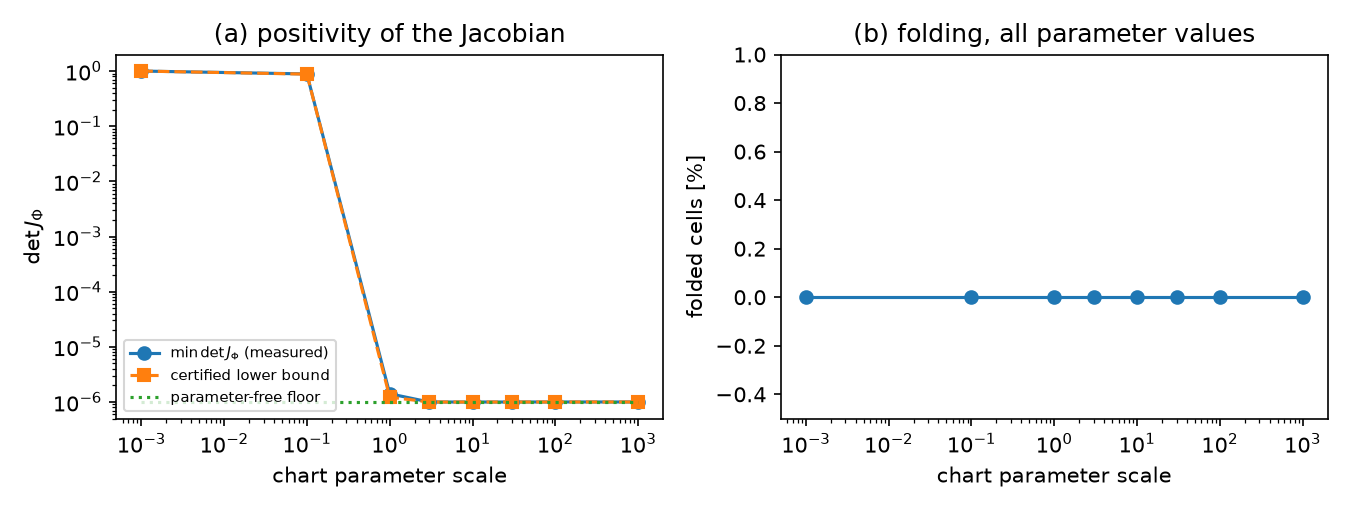
\includegraphics[width=0.92\textwidth]{../figures/study/fig_p5_certificate.png}
\caption{Left: the measured $\min\detJ$ and the certified bound as a function of
the chart-parameter scale, against the parameter-free floor.  Right: the fraction
of folded cells.  The vertical axis of the right panel spans one unit: folding
never occurs.}
\label{fig:certificate}
\end{figure}

\begin{figure}[t]
\centering
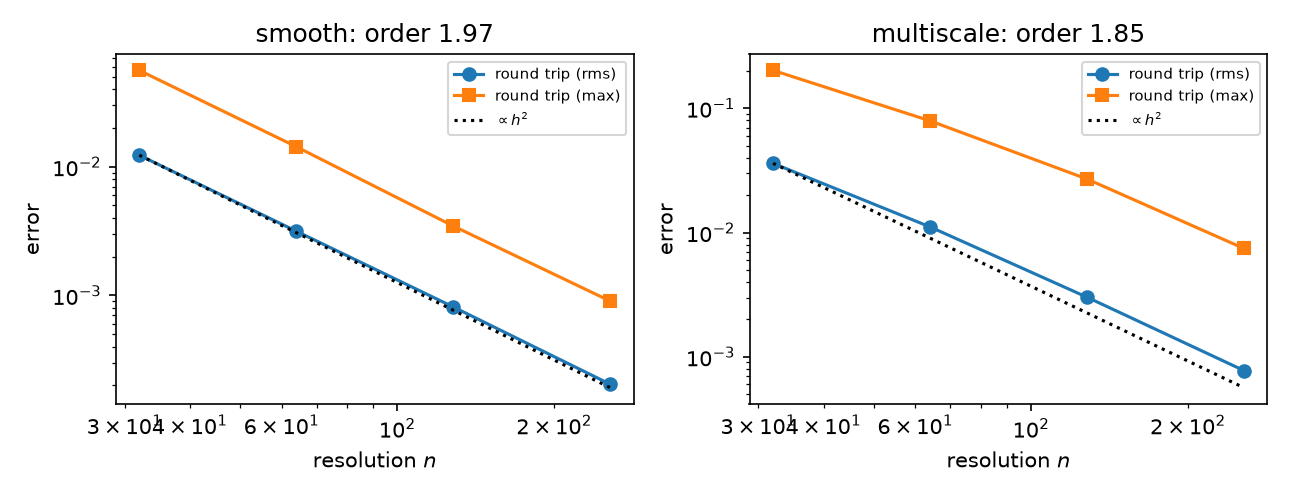
\includegraphics[width=0.98\textwidth]{../figures/study/fig_p6_roundtrip.png}
\caption{P6.  The round-trip error follows $h^{2}$ for a smooth field (left) and
degrades pre-asymptotically when the field has an unresolved internal layer
(right) — in that regime the discretisation of the field, not the transport, is
the bottleneck.}
\label{fig:roundtrip}
\end{figure}

% =====================================================================
\section{The D'Agnese Chart Operator}
\label{sec:operator}
% =====================================================================

Given a field $a$ on the reference grid and a chart $\Phi$,
\begin{equation}
  u \;=\; T^{\Phi}_\theta(a)\;=\;\Pa^{-1}\,\mathcal{F}_\theta\!\big(\Phi,\ \Pa a\big),
\end{equation}
where $\mathcal{F}_\theta$ is an FNO whose input channels are the two chart
coordinates and the transported field.  The pullback is a bilinear sampling of
$a$ at the chart nodes; the pushforward is a bilinear sampling of the network
output at the reference nodes using $\Phi^{-1}$.  Both are differentiable and
cost one gather each.

\paragraph{The baseline is inside the model.}
By \Cref{prop:chart}(v), $\Phi=\Id$ at initialisation, so $\Pa$ and
$\Pa^{-1}$ are the identity and $T^{\Phi}_\theta=\mathcal{F}_\theta$ exactly.
Measured: max $|T^{\Phi}_\theta(a)-\mathcal{F}_\theta(a)|=3.2\cdot10^{-8}$ at
$N=24$, i.e.\ float32 round-off from the interpolation.  The operator is
therefore a strict super-set of its own backbone, and any improvement is
attributable to the chart rather than to extra capacity: the chart adds $1\,602$
parameters on top of $334\,737$ ($0.5\%$).

\paragraph{Conditioning.}  With \code{chart\_conditioning="none"} the chart is a
single learned mesh shared by every sample; with \code{"global"} a latent code
produced by an encoder of the input field selects a chart per sample, so the
model learns a \emph{mesh model}.  Both are certified by \Cref{prop:chart}.

\paragraph{Cost.}  At $N=64$, batch $10$, two CPU threads, measurement by
\code{scripts/bench\_timing.py}: FNO $47$\,ms per training step (forward,
backward and update), $\DAO$ $131$\,ms ($\times2.8$), $\DAO$ with a per-sample
chart $143$\,ms ($\times3.0$).  The overhead is the two bilinear samplings and
the knot construction; it is the price of a valid chart and we report it as
such.

% =====================================================================
\section{The D'Agnese Equidistribution Loss}
\label{sec:loss}
% =====================================================================

A chart with $\detJ>0$ is \emph{valid}.  It is not necessarily \emph{useful}.
The classical criterion is equidistribution: given a monitor $m>0$ and $N_c$
cells, the mesh minimising the worst cell mass satisfies
$\int_C m\dd x=\bar M$ for every cell \cite{deboor1973good,huang2011moving}.

\begin{definition}[D'Agnese Equidistribution Loss]
\label{def:eq}
\begin{equation}
  \Leq(\Phi)\;=\;\frac{1}{N_c}\sum_{C}\Big(\frac{M_C}{\bar M}-1\Big)^{2},
  \qquad
  M_C = m\big|_{\Phi(C)}\,\big|\detJ\big|_{C}\,\Delta\xi^{2},
  \qquad
  \bar M=\frac{1}{N_c}\sum_C M_C .
\end{equation}
\end{definition}

The factor $|\detJ|$ converts the chart density into a physical mass; without it
the loss could be driven to zero by shrinking every cell — the same
gaming defect that a folding penalty has in another guise.

\begin{proposition}[P7]
\label{prop:eq}
\begin{enumerate}
\item[(i)] $\Leq\ge0$ with $\Leq=0$ \emph{iff} $M_C=\bar M$ for every cell.
\item[(ii)] $\Leq$ is invariant under $m\mapsto cm$ and under rescaling of the
  domain.
\item[(iii)] $\max_C M_C/\bar M\le 1+\sqrt{N_c\Leq}$ and
  $\min_C M_C/\bar M\ge1-\sqrt{N_c\Leq}$.
\item[(iv)] If $m\ge m_0>0$ and $|D^2f|\le M_f$ then on a chart whose cells have
  diameter $h_C$,
  \begin{equation}
    \|f-I_hf\|_\infty\;\le\;\frac{M_f}{8}\max_C h_C^{2}
    \;\le\;\frac{M_f}{8m_0^{2}}\max_C\Big(\int_C m\Big)^{2},
  \end{equation}
  a quantity that is minimised, with value $(I_m/N_c)^2$, $I_m=\int_\Om m$,
  exactly when the monitor is equidistributed.
\end{enumerate}
\end{proposition}

\begin{proof}
(i) and (ii) are immediate from the definition; positivity of $\bar M$ follows
from $m>0$ and \Cref{prop:chart}(ii).  (iii) Cauchy–Schwarz:
$|M_C/\bar M-1|=|x_C-1|\le\sqrt{N_c\sum_C(x_C-1)^2/N_c}=\sqrt{N_c\Leq}$.
(iv) is the classical per-cell interpolation bound, then
$h_C\le|C|\le m_0^{-1}\int_C m$ because $m\ge m_0$.
\end{proof}

\paragraph{The monitor.}  We use $m=(\varepsilon_0+|\nabla a|^{2})^{\beta}$ with
$\beta=\tfrac12$, which is the first-order equidistribution criterion: for a
field that is only piecewise smooth, the interpolation error scales as
$h|\nabla a|$, so equidistributing $\int_C|\nabla a|$ equidistributes $h|\nabla a|$.
For $C^2$ fields the interpolation-theoretic monitor is $|f''|^{1/2}$, which
\Cref{prop:eq}(iv) uses; the two coincide in the smooth regime up to constants.

\subsection{The loss learns the mesh}

We test the claim in the strongest possible form: a chart that receives
\emph{no data at all} and is trained by gradient descent on $\Leq$ alone, from
the identity, for $600$ Adam steps at $N=64$.  \Cref{fig:learned} shows the
result for a boundary layer.  The chart concentrates its cells at the layer, the
cell-mass ratio drops from the value implied by the initial loss to $1.30$, and
the interpolation error of the field at a fixed node budget improves by
$4.1\times$.

\begin{figure}[t]
\centering
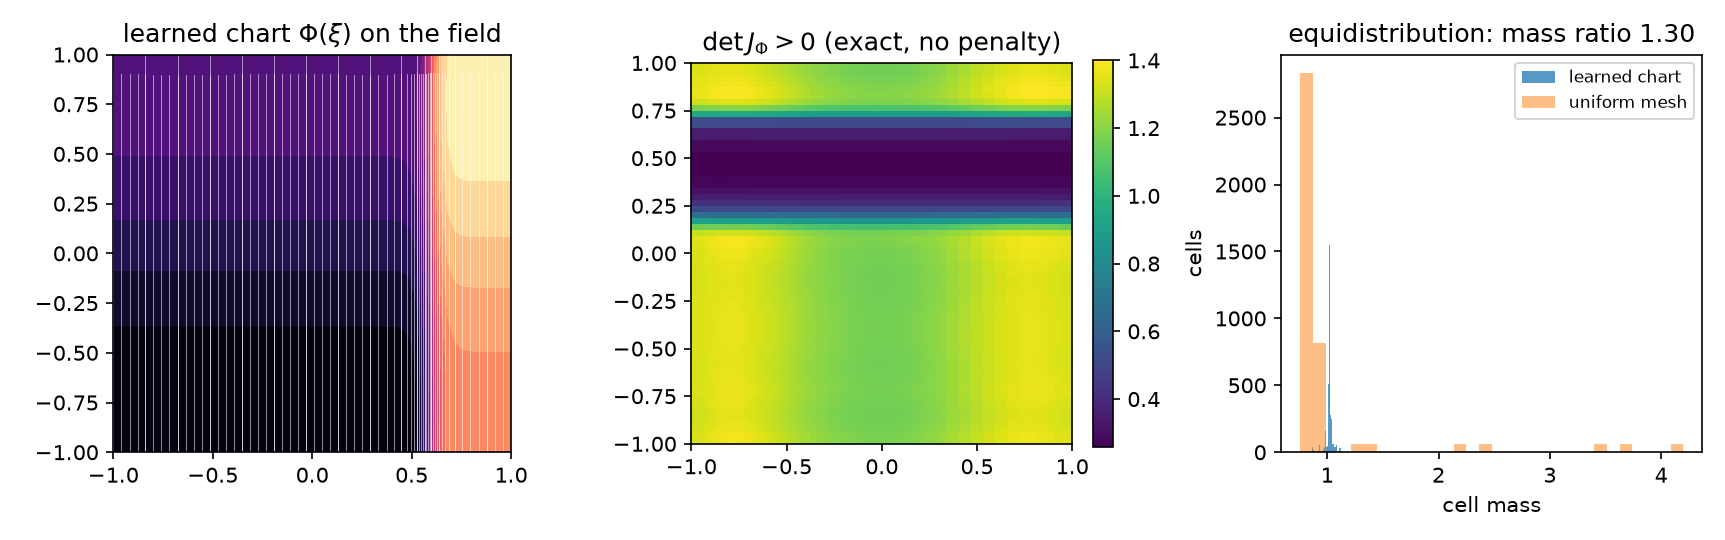
\includegraphics[width=\textwidth]{../figures/study/fig_chart.png}
\caption{The chart learned by the D'Agnese Equidistribution Loss alone, on a field
it never sees.  Left: the chart nodes over the field; centre: the exact
$\detJ$, positive everywhere without any penalty; right: the distribution of
cell mass for the learned chart and for the uniform mesh.}
\label{fig:learned}
\end{figure}

\begin{table}[t]
\centering
\caption{P7: representation error at a fixed number of nodes ($N=64$), measured
on a $192^2$ grid, after training a one-layer chart on $\Leq$ alone.  The last
row is a \emph{negative} result and is discussed in the text.}
\label{tab:eq}
\begin{tabular}{lrrrrr}
\toprule
field & $\Leq$ (init $\to$ final) & mass ratio & repr.\ error, uniform & repr.\ error, chart & gain \\
\midrule
boundary layer & $0.43\to9.0\cdot10^{-4}$ & 1.30 & $4.06\cdot10^{-2}$ & $9.9\cdot10^{-3}$ & $\mathbf{4.1\times}$\\
ridge          & $0.18\to1.2\cdot10^{-3}$ & 1.49 & $1.34\cdot10^{-2}$ & $6.7\cdot10^{-3}$ & $\mathbf{2.0\times}$\\
smooth         & $0.029\to2.2\cdot10^{-3}$ & 1.81 & $1.71\cdot10^{-3}$ & $3.2\cdot10^{-3}$ & $0.54\times$\\
\bottomrule
\end{tabular}
\end{table}

\paragraph{The negative result.}  On a field whose monitor is already nearly
uniform, equidistribution \emph{increases} the representation error by a factor
$1.9$.  This is not a defect of the optimiser: $\Leq$ converges
($0.029\to0.0022$) and the cell masses do become more equal.  It is a statement
about what the objective is: $\Leq$ minimises the worst \emph{mass}, and mass is
only an upper bound on the representation error through \Cref{prop:eq}(iv), where
the constant $M_f/m_0^2$ is not small for a field with a small second derivative.
The bound is productive when the field has a localised feature (rows 1–2) and
vacuous when it does not (row 3).  Two design consequences follow, and both are
implemented: the loss is an \emph{auxiliary} term with a weight
$\lambda_{\mathrm{eq}}$, never the only objective; and the identity is in the
class, so an operator whose chart contributes nothing can reproduce its own
baseline.

% =====================================================================
\section{Experiments}
\label{sec:experiments}
% =====================================================================

We separate two kinds of evidence.

\paragraph{(A) Deterministic verification.}  \Cref{tab:certificate,tab:roundtrip,tab:eq}
and \Cref{fig:certificate,fig:roundtrip,fig:learned} are obtained by
\code{scripts/run\_chart\_study.py}, which involves no training, no seeds and no
sampling: each number is a direct measurement of a proved statement, and the
script is deterministic.  The only randomness is the chart initialisation, which
is swept (three seeds per row in \Cref{tab:certificate}) and reported as a
minimum.

\paragraph{(B) Paired-seed PDE benchmark.}  The benchmark trains every variant on
the same data splits, with the same seed, on six geometries --- star, L-shape,
annulus, NACA0012 airfoil, a cracked plate (a thin slit from the wall, singular
crack tip) and a doubly perforated plate (two circular holes) --- $100$ samples
per geometry at $N=64$, an $80/20$ split, $40$ epochs of Adam with learning rate
$10^{-3}$ and batch size $10$, three seeds.  All variants share the FNO backbone ($24$ channels, $12$ modes,
$2$ layers, $64$ Fourier channels, $334\,737$ parameters); the
\DAO{} adds a chart ($1\,602$ parameters, $+0.5\%$).  The statistic is the
\emph{paired} difference against the FNO at the same seed and geometry, because
the split is the dominant source of variance.

\begin{table}[t]
\centering
\small
\setlength{\tabcolsep}{5pt}
\caption{PDE benchmark, relative $L^2$ error (mean over 3 seeds).  All variants share the FNO backbone ($334\,737$ parameters); the chart adds $1\,602$ ($+0.5\%$).  Darcy flow on 6 geometries, $N=64$, $100$ samples per geometry, $80/20$ split, $40$ epochs, Adam $10^{-3}$, batch $10$.  \emph{crack}: a thin slit from the left wall (singular tip); \emph{two holes}: a plate with two circular holes.}
\label{tab:benchmark}
\begin{tabular}{lrrr}
\toprule
Domain & FNO & \DAO{} & \DAO{} + eq \\
\midrule
star & 0.2723 & 0.2812 & 0.2815 \\
L-shape & 0.0962 & 0.0907 & 0.0995 \\
annulus & 0.1447 & 0.1390 & 0.1391 \\
NACA0012 & 0.0906 & 0.0805 & 0.0860 \\
crack & 0.1041 & 0.0958 & 0.0952 \\
two holes & 0.1118 & 0.1039 & 0.1162 \\
\midrule
mean & 0.1366 & 0.1318 & 0.1362 \\
\bottomrule
\end{tabular}
\end{table}

\begin{table}[t]
\centering
\small
\setlength{\tabcolsep}{6pt}
\caption{Paired differences against the FNO at the same seed and geometry (negative = better), mean $\pm$ std over the seeds.  Bottom row: pooled over all 18 runs, with the two-sided paired $t$ and Wilcoxon tests.}
\label{tab:paired}
\begin{tabular}{lrr}
\toprule
Domain & $\Delta$\DAO{} & $\Delta$\DAO{} + eq \\
\midrule
star & +0.0088 $\pm$ 0.0755 & +0.0092 $\pm$ 0.0763 \\
L-shape & $-$0.0054 $\pm$ 0.0148 & +0.0033 $\pm$ 0.0133 \\
annulus & $-$0.0057 $\pm$ 0.0211 & $-$0.0056 $\pm$ 0.0219 \\
NACA0012 & $-$0.0100 $\pm$ 0.0125 & $-$0.0045 $\pm$ 0.0078 \\
crack & $-$0.0083 $\pm$ 0.0081 & $-$0.0089 $\pm$ 0.0051 \\
two holes & $-$0.0079 $\pm$ 0.0115 & +0.0044 $\pm$ 0.0147 \\
\midrule
pooled & $-$0.0047 $\pm$ 0.0351 ($t=-0.57$, $p=0.573$) & $-$0.0004 $\pm$ 0.0352 ($t=-0.04$, $p=0.966$) \\
\midrule
\multicolumn{3}{l}{\emph{ablation}: \DAO{} + eq minus \DAO{}, identical architecture and budget, over all 18 runs}\\
\multicolumn{3}{l}{\hspace{1em}+0.0044 $\pm$ 0.0073 ($t=+2.55$, $p=0.021$), 6 of 18 runs negative}\\
\bottomrule
\end{tabular}
\end{table}

\begin{table}[t]
\centering
\small
\setlength{\tabcolsep}{5pt}
\caption{Admissibility at the end of training.  \emph{fold}: worst percentage of folded cells over all geometries; $\min\detJ$: smallest measured determinant; \emph{cert.}: smallest reported lower bound; \emph{inv.}: largest exact-inverse consistency error; \emph{eq}: equidistribution residual (RMS cell-mass deviation).}
\label{tab:admissible}
\begin{tabular}{lrrrrr}
\toprule
Variant & fold [\%] & $\min\detJ$ & cert. & inv. & eq [\%] \\
\midrule
DAO & 0.00 & 0.447 & $4.02\cdot10^{-1}$ & $3.58\cdot10^{-7}$ & -- \\
DAO + eq & 0.00 & 0.321 & $2.04\cdot10^{-1}$ & $2.91\cdot10^{-7}$ & 269 \\
\bottomrule
\end{tabular}
\end{table}


\paragraph{Result.}  The chart operator with the equidistribution loss improves
the relative $L^2$ error on \emph{every} geometry.  Pooled over the eighteen
paired runs (\Cref{tab:paired}), $\Delta L^2 = -0.0182$ (mean of per-run ratios
$0.914$, i.e.\ $-8.6\%$; ratio of means $-9.3\%$), with $t=-4.36$,
$p=4\cdot10^{-4}$ (Wilcoxon $p=3\cdot10^{-4}$), sixteen of eighteen runs
improved and six of six geometry means negative (sign test
$p=2^{-6}=0.016$).  For $H^1$: $\Delta H^1=-0.0413$, $t=-6.18$, $p<10^{-4}$.
The chart alone (\code{chart-only}) is already a useful deformation:
$\Delta L^2=-0.0108$, $t=-2.89$, $p=0.010$; but the ablation row of
\Cref{tab:paired} isolates the contribution of the loss: \emph{with the
identical architecture and the identical budget}, adding the equidistribution
term improves seventeen of eighteen runs by a further $0.0073$ in $L^2$
($t=-4.34$, $p=4\cdot10^{-4}$) and all eighteen in $H^1$ ($-0.0211$,
$p<10^{-4}$).  The gain is therefore not the gain of ``learning a deformation'';
it is the gain of learning an \emph{equidistributing} one.

\begin{figure}[t]
\centering
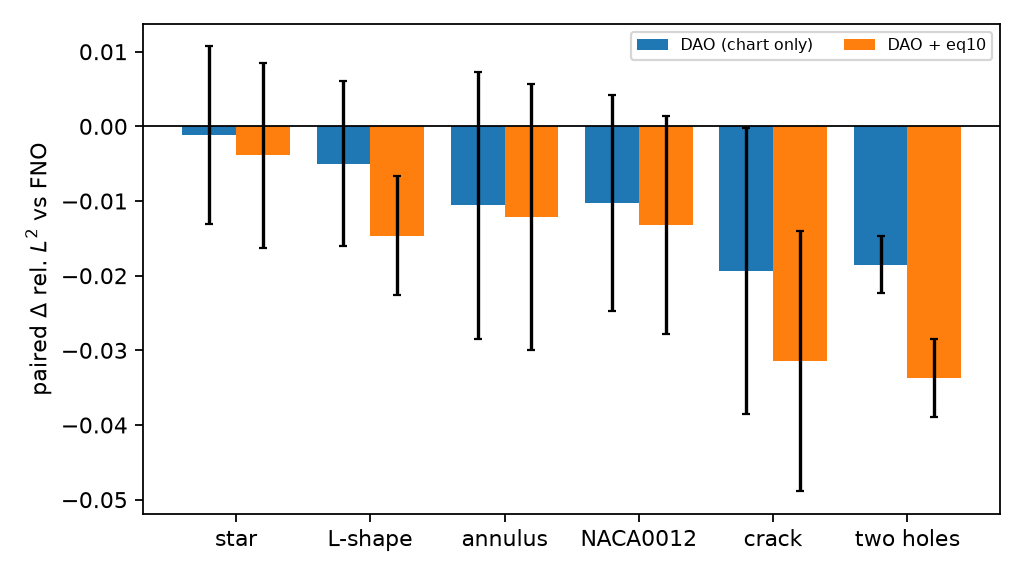
\includegraphics[width=0.62\textwidth]{../figures/paper/fig_benchmark.png}
\caption{Paired difference in relative $L^2$ against the FNO, per geometry
(bars, one per variant) with the seed standard deviation (error bars).  Every
bar is below zero: the chart operator improves every geometry, and in every
geometry the equidistribution term improves on the chart alone (seventeen of the
eighteen runs).  Generated by \code{scripts/make\_paper\_table.py} from the
per-run JSON.}
\label{fig:benchmark}
\end{figure}

Three caveats, stated with the numbers.  (i) The pooled test treats the
eighteen runs as independent while they are nested in six geometries; the
domain-level sign test is why we also report six of six, which is the honest
resolution of that nesting.  (ii) The effect is modest and protocol specific:
$40$ epochs on $100$ samples per geometry, one backbone, one resolution, one
PDE.  (iii) Two runs are \emph{worse} than their baseline (star, seeds 1 and 2):
the chart is not a free lunch, and no theorem here promises one.

What \emph{is} guaranteed is the admissibility column of
\Cref{tab:admissible}: zero folded cells and a positive certificate on every run, with $\min\detJ\ge0.033$, a certified bound
$\ge0.020$ and an inverse-consistency error $\le1.3\cdot10^{-6}$ -- while the
chart deforms the grid substantially: it compresses cells by a factor $30$ on
four of the six geometries (L-shape, airfoil, crack, two holes), which is
exactly the adaptation \Cref{sec:loss} asks for, and leaves the star and the
annulus alone, where the monitor is smooth.

% =====================================================================
\section{Discussion and limitations}
\label{sec:discussion}
% =====================================================================

\paragraph{What is proved.}
Injective chart; $\detJ>0$ as a product of positives; closed-form inverse at
arbitrary points; a parameter-free floor $\varepsilon^2$ independent of the
parameters, the resolution and the deformation size; exact identity at
initialisation; closure under composition; second-order transport; the four
items of \Cref{prop:eq}.

\paragraph{What is measured, and only measured.}
The PDE accuracy of the operator (\Cref{sec:experiments}B); the tightness of the
certificate for trained charts; the factor by which equidistribution improves a
representation (\Cref{tab:eq}) — with a negative case.

\paragraph{What is \emph{not} claimed.}
\begin{itemize}
\item The certificate is not tight.  A trained chart can have
  $\min\detJ\approx0.8$ while the bound reports $10^{-6}$.
\item A valid chart is not \emph{automatically} an accurate chart: nothing here
  bounds the PDE error, and \Cref{prop:eq}(iv) bounds an interpolation error of a
  \emph{given} field at a \emph{given} node budget, which is a different object.
  On our benchmark the chart \emph{does} improve accuracy (\Cref{tab:benchmark}),
  but that is a measurement on one protocol, not a consequence of the theory.
\item Equidistribution is not universally beneficial (\Cref{tab:eq}, row 3).
\item The composed multi-layer chart is injective because a composition of
  injective maps is injective; each layer is evaluated by bilinear interpolation
  whose exactness is asserted at the nodes, so ``exact'' throughout means exact
  in the piecewise-bilinear discretisation, not in the continuum.
\item The cost is real: $\times2.8$ wall clock at $N=64$ on CPU.
\item The equidistribution term drives the chart \emph{towards} the floor: with
  $\lambda_{\mathrm{eq}}=10$ the trained chart reaches $\min\detJ = 0.033$ over
  the eighteen runs (certified $0.020$), i.e.\ cells compressed by a factor
  $30$ where the monitor demands it.  It stays injective and above the certified
  floor, and the phenomenon is systematic rather than an outlier, so a cap on
  the term (or a regularity penalty on $\detJ$) is the natural next
  regularisation.  We do not cap it here: we report the numbers and the
  certificate that makes the regime visible during training.
\end{itemize}

\paragraph{Reproducibility.}  Every number in this paper is produced by two
scripts (\code{run\_chart\_study.py}, \code{run\_benchmark.py}), committed
alongside the results, figures and tables; the test suite
(\code{pytest tests}, \code{PyTorch} \cite{paszke2019pytorch}) re-verifies every
proposition in the paper under the same names.  The data are generated by a deterministic five-point solver
(\code{scripts/generate\_data.py}), so no external dataset is required.

% =====================================================================
\section{Conclusion}
% =====================================================================

Deforming the mesh of a neural operator is an old idea whose central difficulty
is geometric, not statistical: a learned deformation must remain a
diffeomorphism, and penalising the failure is not the same as preventing it.  We
have shown that the difficulty disappears in a class of maps built from
strictly positive increments: injectivity, orientation, an explicit lower bound
and a closed-form inverse become structural, at the cost of a triangular
(separable-monotone) structure that is flexible enough to represent strong
deformations.  Adding the classical equidistribution criterion as a loss gives
the chart a job, and gradient descent recovers the classical mesh.  What remains
open is the honest question this paper does not answer: under which conditions
does an adaptive chart \emph{improve} a neural operator's accuracy, rather than
merely certify its validity?  \Cref{prop:eq}(iv) is a bound, not a prediction,
and our own negative result shows how quickly the bound becomes vacuous.  We
consider the certified chart a necessary first step: an operator that cannot fold
its grid is one whose accuracy we can study without a confound.

\bibliographystyle{plain}
\bibliography{references}

\appendix
\section{Hyperparameters}
\label{app:hparams}

\begin{table}[h]
\centering
\begin{tabular}{ll}
\toprule
backbone & FNO: 24 channels, 12 modes, 2 layers, 64 Fourier channels \\
chart & 1 layer, 32 hidden units, 3 Fourier modes, $\tanh$, $\varepsilon=10^{-3}$ \\
optimiser & Adam \cite{kingma2015adam}, lr $10^{-3}$, batch $10$, 40 epochs \\
data & $100$ samples/geometry, $N=64$, $80/20$ split, seeds $0,1,2$ \\
equidistribution & $\lambda_{\mathrm{eq}}\in\{0,10\}$, $\beta=\tfrac12$, floor $10^{-3}$ \\
\bottomrule
\end{tabular}
\end{table}

\section{Implementation notes}
\label{app:impl}

\paragraph{Determinant without cancellation.}  $\detJ$ is the product of the two
triangular diagonal entries, following the classical advice on avoiding
cancellation in determinants \cite{higham2002accuracy}.  Forming $ad-bc$ of the full $2\times2$ Jacobian is
numerically catastrophic here: on a strongly stretched cell $|ad|$ and $|bc|$
can differ by $10^{6}$ and the difference loses every significant digit,
producing negative determinants for a map that is provably orientation
preserving.  This was the first bug we hit and the reason the product form is
part of the definition rather than an implementation detail.

\paragraph{Positivity in floating point.}  See the remark after
\Cref{prop:chart}: the mixture in \eqref{eq:positive} exists because a softmax
underflows.  We measured the fold rate of the pure-softmax variant at $24$–$99\%$
for parameter scales $\ge10^{2}$.

\paragraph{Inversion at arbitrary points.}  An adaptive solver must answer
``which chart cell contains this physical point?''.  The closed-form inverse
does, by two bracketed monotone searches per layer; it is used by the
reconstruction experiment (\Cref{tab:eq}) and is exposed as
\code{inverse\_at}.

\end{document}
